\documentclass[12pt]{article}

\usepackage{sbc-template}

\usepackage{graphicx,url}

\usepackage[brazil]{babel}   
\usepackage[utf8]{inputenc}  

     
\sloppy

\title{Projeto Integrador II\\ Título provisório}

\author{Alexandre S. Bencz\inst{1}, Ezequiel F. Santos\inst{1}, Gabriel Fontenelle\inst{1}, Tales Pádua\inst{1} }

\address 
{Centro Universitário SENAC - Campus Santo Amaro
  (SENAC-SP)\\
  Av. Engenheiro Eusébio Stevaux, 823 -- Santo Amaro, São Paulo -- CEP 04696-000 -- SP -- Brasil
%\nextinstitute
%  Departamento de Tecnologia da Informação\\
%  Bacharelado em Ciência da Computação
  \email{{alebencz,ezefranca.br,colecionador.gabriel,talescpadua},{(@gmail.com})}
}

\begin{document} 

\maketitle

\begin{abstract}
Space reservation for translation, when resumo is final version % if you want translate, go ahead
\end{abstract}
     
\begin{resumo} 
  Este meta-artigo descreve o trabalho relativo ao desenvolvimento de 
  um jogo educativo para o ensino de lógica boolena. 
  Neste trabalho foi elaborado em game 2D isométrico utilizando
  a biblioteca Allegro5 e a linguagem C. 
  Prentende-se descrever a elaboração do mesmo, 
  passando pelos seus aspectos técnicos, recursos pedagógicos e 
  lúdicos utilizados e por fim seu resultado final.
\end{resumo}


\section{Introdução}

\section{Desenvolvimento de um jogo educativo} \label{sec:gamedev}

\section{Estado da Arte}

\subsection{Jogos Educativos}
\subsection{Elementos pedagógicos e lúdicos dos jogos}
\subsection{Desenvolvimento de jogos 2D isométricos}
\subsection{A biblioteca allegro, cases e exemplos}



\section{Elaboração pedagógica e elementos lúdicos}

O significado atual do jogo na educação, sinaliza a existência  de divergências em torno do jogo educativo, que estaria relacionado concomitamente a duas funções.\cite[kishimoto:08]
A primeira seria a função lúdica do jogo, expressa na idéia de que sua vivência propicia a diversão, o prazer, quando escolhido voluntariamente pelo individuo. A segunda seria a função

\section{Elaboração técnica}


\subsection{Biblioteca Allegro5}

Utilização da biblioteca allegro5

\subsection{Desenvolvimento de uma Engine utilizando structs}

Maquinas de estado finito, "simulação de orientação a objeto em c"

\section{Imagens do Jogo}\label{sec:figs}


Figure and table captions should be centered if less than one line
(Figure~\ref{fig:exampleFig1}), otherwise justified and indented by 0.8cm on
both margins, as shown in Figure~\ref{fig:exampleFig2}. The caption font must
be Helvetica, 10 point, boldface, with 6 points of space before and after each
caption.

\begin{figure}[ht]
\centering
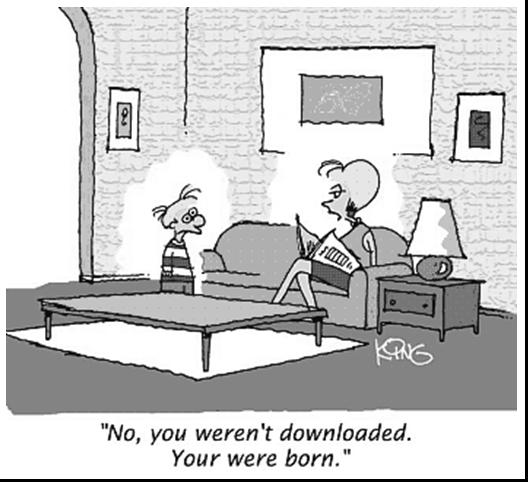
\includegraphics[width=.5\textwidth]{fig1.jpg}
\caption{A typical figure}
\label{fig:exampleFig1}
\end{figure}

\begin{figure}[ht]
\centering
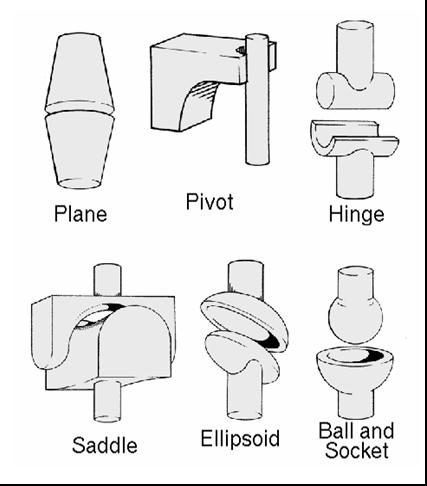
\includegraphics[width=.3\textwidth]{fig2.jpg}
\caption{This figure is an example of a figure caption taking more than one
  line and justified considering margins mentioned in Section~\ref{sec:figs}.}
\label{fig:exampleFig2}
\end{figure}

In tables, try to avoid the use of colored or shaded backgrounds, and avoid
thick, doubled, or unnecessary framing lines. When reporting empirical data,
do not use more decimal digits than warranted by their precision and
reproducibility. Table caption must be placed before the table (see Table 1)
and the font used must also be Helvetica, 10 point, boldface, with 6 points of
space before and after each caption.

\begin{table}[ht]
\centering
\caption{Variables to be considered on the evaluation of interaction
  techniques}
\label{tab:exTable1}
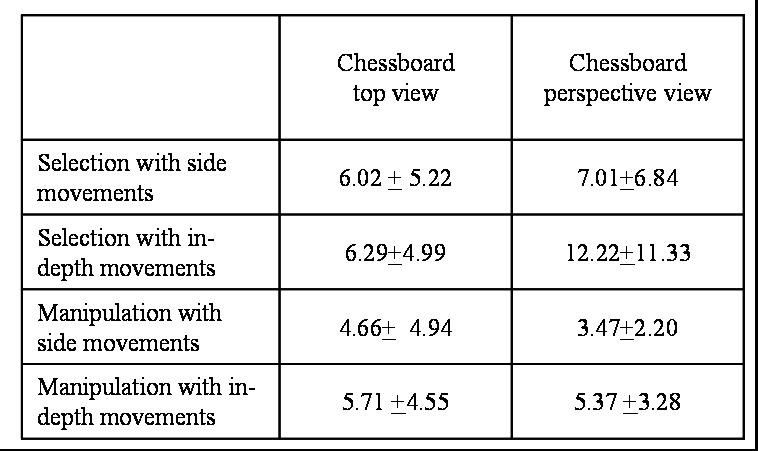
\includegraphics[width=.7\textwidth]{table.jpg}
\end{table}

\section{Conclusão}

A Conclusão só poderá ser elaborada ao fim das atividades do projeto integrador, pois não é possível concluir sem ter feito ou sem saber, claro que você encontrará pelo mundo afora gerentes que concluem tudo sem saber nada, é uma coisa típica dos humanos, pessoas idiotas assumindo cargos de poder, diferente da meritocracia real do mundo animal, onde o poder está com aqueles que possuem qualidades superiores.

\section{References}

Para fazer uma citação pode usar assim \cite{barbosa:97},
\cite{rau:11}, \cite{barbosa:97}.

SÓ LEMBRE DE ADICIONAR A BIBLIOGRAFIA CERTINHA NO ARQUIVO *.bib

\bibliographystyle{sbc}
\bibliography{sbc-template}

\end{document}
